%\right \right \right \right \right \right \right \right \right \right \right \right \right \right \right \right \right \right \right \right \right \right \right \right \right \right \right \right \right \right \right \right \right \right \right \right \right \right \right \right \right \right \right \right \right \right \right \right \right 	~~~~~~~~```% This is "sig-alternate.tex" V2.0 May 2012
% This file should be compiled with V2.5 of "sig-alternate.cls" May 2012
%
% This example file demonstrates the use of the 'sig-alternate.cls'
% V2.5 LaTeX2e document class file. It is for those submitting
% articles to ACM Conference Proceedings WHO DO NOT WISH TO
% STRICTLY ADHERE TO THE SIGS (PUBS-BOARD-ENDORSED) STYLE.
% The 'sig-alternate.cls' file will produce a similar-looking,
% albeit, 'tighter' paper resulting in, invariably, fewer pages.
%
% ----------------------------------------------------------------------------------------------------------------
% This .tex file (and associated .cls V2.5) produces:
%       1) The Permission Statement
%       2) The Conference (location) Info information
%       3) The Copyright Line with ACM data
%       4) NO page numbers
%
% as against the acm_proc_article-sp.cls file which
% DOES NOT produce 1) thru' 3) above.
%
% Using 'sig-alternate.cls' you have control, however, from within
% the source .tex file, over both the CopyrightYear
% (defaulted to 200X) and the ACM Copyright Data
% (defaulted to X-XXXXX-XX-X/XX/XX).
% e.g.
% \CopyrightYear{2007} will cause 2007 to appear in the copyright line.
% \crdata{0-12345-67-8/90/12} will cause 0-12345-67-8/90/12 to appear in the copyright line.
%
% ---------------------------------------------------------------------------------------------------------------
% This .tex source is an example which *does* use
% the .bib file (from which the .bbl file % is produced).
% REMEMBER HOWEVER: After having produced the .bbl file,
% and prior to final submission, you *NEED* to 'insert'
% your .bbl file into your source .tex file so as to provide
% ONE 'self-contained' source file.
%
% ================= IF YOU HAVE QUESTIONS =======================
% Questions regarding the SIGS styles, SIGS policies and
% procedures, Conferences etc. should be sent to
% Adrienne Griscti (griscti@acm.org)
%
% Technical questions _only_ to
% Gerald Murray (murray@hq.acm.org)
% ===============================================================
%
% For tracking purposes - this is V2.0 - May 2012

\documentclass{sig-alternate}
\usepackage[normalem]{ulem}
\usepackage{algpseudocode}
\usepackage{algorithm}

\usepackage{algorithm,algpseudocode}
\makeatletter
\newcommand{\StatexIndent}[1][3]{%
  \setlength\@tempdima{\algorithmicindent}%
  \Statex\hskip\dimexpr#1\@tempdima\relax}
\algdef{S}[WHILE]{WhileNoDo}[1]{\algorithmicwhile\ #1}%
\makeatother


\usepackage{amsmath}
%\usepackage{url}
\usepackage{graphicx}
\usepackage{subfigure}
\usepackage{multirow}
 \usepackage{url}

\usepackage{footnote}
\makesavenoteenv{tabular}
\makesavenoteenv{table}

\algrenewcommand{\algorithmicrequire}{\textbf{Input:}}
\algrenewcommand{\algorithmicensure}{\textbf{Output:}}
\renewcommand{\algorithmicforall}{\textbf{for each}}

\begin{document}
%
% --- Author Metadata here ---
\conferenceinfo{WOODSTOCK}{'97 El Paso, Texas USA}
%\CopyrightYear{2007} % Allows default copyright year (20XX) to be over-ridden - IF NEED BE.
%\crdata{0-12345-67-8/90/01}  % Allows default copyright data (0-89791-88-6/97/05) to be over-ridden - IF NEED BE.
% --- End of Author Metadata ---

\title{An interleaving approach to combinatorial testing and failure-inducing interaction identification\titlenote{This work was supported by the National Natural Science Foundation of China (No. 61272079), the Research Fund for the Doctoral Program of Higher Education of China (No.20130091110032), the Science Fund for Creative Research Groups of the National Natural Science Foundation of China(No. 61321491), and the Major Program of National Natural Science Foundation of China (No. 91318301)}
}
%
% You need the command \numberofauthors to handle the 'placement
% and alignment' of the authors beneath the title.
%
% For aesthetic reasons, we recommend 'three authors at a time'
% i.e. three 'name/affiliation blocks' be placed beneath the title.
%
% NOTE: You are NOT restricted in how many 'rows' of
% "name/affiliations" may appear. We just ask that you restrict
% the number of 'columns' to three.
%
% Because of the available 'opening page real-estate'
% we ask you to refrain from putting more than six authors
% (two rows with three columns) beneath the article title.
% More than six makes the first-page appear very cluttered indeed.
%
% Use the \alignauthor commands to handle the names
% and affiliations for an 'aesthetic maximum' of six authors.
% Add names, affiliations, addresses for
% the seventh etc. author(s) as the argument for the
% \additionalauthors command.
% These 'additional authors' will be output/set for you
% without further effort on your part as the last section in
% the body of your article BEFORE References or any Appendices.

\numberofauthors{3} %  in this sample file, there are a *total*
% of EIGHT authors. SIX appear on the 'first-page' (for formatting
% reasons) and the remaining two appear in the \additionalauthors section.
%
\author{
% You can go ahead and credit any number of authors here,
% e.g. one 'row of three' or two rows (consisting of one row of three
% and a second row of one, two or three).
%
% The command \alignauthor (no curly braces needed) should
% precede each author name, affiliation/snail-mail address and
% e-mail address. Additionally, tag each line of
% affiliation/address with \affaddr, and tag the
% e-mail address with \email.
%
% 1st. author
%\and
%\alignauthor
 Xintao Niu and Changhai Nie\\
       \affaddr{State Key Laboratory for Novel}\\
       \affaddr{ Software Technology}\\
       \affaddr{Nanjing University}\\
       \affaddr{China, 210023}\\
    %   \email{niuxintao@gmail.com}\\
       \email{changhainie@nju.edu.cn}\\
% 2nd. author
%\alignauthor
%Changhai Nie \\
% \affaddr{State Key Laboratory for Novel}\\
%       \affaddr{ Software Technology}\\
%       \affaddr{Nanjing University}\\
%       \affaddr{China, 210023}\\
%       \email{changhainie@nju.edu.cn}
\alignauthor
Hareton Leung \\
       \affaddr{Department of computing}\\
       \affaddr{Hong Kong Polytechnic University}\\
       \affaddr{Kowloon, Hong Kong}\\
       \email{cshleung@comp.polyu.edu.hk}
\alignauthor
Jeff Lei \\
       \affaddr{Department of Computer}\\
       \affaddr{Science and Engineering }\\
       \affaddr{The University of Texas at Arlington}\\
%       \affaddr{Arlington, Texas}\\
       \email{ylei@cse.uta.edu}
\and
% 3rd. author'
%\alignauthor
%Jeff Lei\\
% 3rd. author'
%\and
\alignauthor
JiaXi Xu and Yan Wang  \\
       \affaddr{ School of Information Engineering}\\
       \affaddr{Nanjing Xiaozhuang University}\\
       \affaddr{China, 211171}\\
       \email{xujiaxi@njxzc.edu.cn} \\
       %\email{wangyan@njxzc.edu.cn}
\alignauthor
%Yan Wang\\
%       \affaddr{ School of Information Engineering}\\
%       \affaddr{Nanjing Xiaozhuang University}\\
%       \affaddr{China, 211171}\\
%%       \email{xujiaxi@njxzc.edu.cn} \\
%       \email{wangyan@njxzc.edu.cn}
%\alignauthor
Xiaoyin Wang \\
       \affaddr{Department of Computer Science}\\
       \affaddr{University of Texas at San Antonio}\\
 %      \affaddr{China, 211171}\\
%       \email{xujiaxi@njxzc.edu.cn} \\
       \email{Xiaoyin.Wang@utsa.edu}
}
% There's nothing stopping you putting the seventh, eighth, etc.
% author on the opening page (as the 'third row') but we ask,
% for aesthetic reasons that you place these 'additional authors'
% in the \additional authors block, viz.
% Just remember to make sure that the TOTAL number of authors
% is the number that will appear on the first page PLUS the
% number that will appear in the \additionalauthors section.
\maketitle
\begin{abstract}
Combinatorial testing(CT) seeks to detect potential faults caused by various interactions of factors that can influence the software systems. When applying CT, it is a common practice to first generate a set of test cases to cover each possible interaction and then to identify the failure-inducing interaction after a failure is detected. Although this conventional procedure is simple and straightforward, we conjecture that it is not the ideal choice in practice. This is because 1) testers desire to identify the root cause of failures before all the needed test cases are generated and executed 2) the early identified failure-inducing interactions can guide the remaining test cases generation, such that many unnecessary and invalid test cases can be avoided. For these reasons, we propose a novel CT framework that allows both generation and identification process to interact with each other. As a result, both generation and identification stages will be done more effectively and efficiently. We conducted a series of empirical studies on several open-source software, the results of which show that our framework can identify the failure-inducing interactions more quickly than traditional approaches, while requiring fewer test cases.

\end{abstract}


\category{D.2.5}{Software Engineering}{Testing and debugging}[Debugging aids,testing tools]

\terms{Reliability, Verification}

\keywords{Software Testing, Combinatorial Testing, Covering Array, Failure-inducing interactions} % NOT required for Proceedings

\section{Introduction}

 Modern software is becoming more and more complex. To test such software is challenging, as the candidate factors that can influence the system's behaviour, e.g., configuration options, system inputs, message events, are enormous. Even worse, the interactions between these factors can also crash the system, e.g., the incompatibility problems. In consideration of the scale of the real industrial software, to test all the possible interactions of all the factors (we call them the interaction space) is not feasible, and even if it is possible, it is not wise to test all the interactions because most of them do not provide any useful information.

Many empirical studies show that, in real software systems, the effective interaction space, i.e., targeting fault detection, makes up only a small proportion of the overall interaction space \cite{kuhn2002investigation,kuhn2004software}. What's more, the number of factors involved in these effective interactions is relatively small, of which 4 to 6 is usually the upper bounds\cite{kuhn2002investigation}. With this observation, applying CT in practice is appealing, as it is proven to be effective to detect the interaction faults in the system.

A typical CT life-cycle is shown in Figure \ref{ct-life}, which contains four main testing stages. At the very beginning of the testing, engineers should extract the specific model of the software under test. In detail, they should identify the factors, such as user inputs, configure options, that could affect the system's behavior. Further effort is needed to figure out the constraints and dependencies between each factor and corresponding values for valid testing. After the modeling stage, a set of test cases should be generated and executed to expose the potential faults in the system. In CT, each test case is a set of assignments of all the factors in the test model. Thus, when such a test case is executed, all the interactions contained in the test case are deemed to be checked. The main target of this stage is to design a relatively small set of test cases to achieve some specific coverage. The third testing stage in this cycle is the fault localization, which is responsible for identifying the failure-inducing interactions. To characterize the failure-inducing interactions of corresponding factors and values is important for future bug fixing, as it will reduce the suspicious code scope to be inspected. The last testing stage of CT is evaluation. In this stage, testers will assess the quality of the previously conducted testing tasks. If the assessment result shows that the previous testing process does not fulfil the testing requirement, some testing stages should be improved, and sometimes, may even need to be re-conducted.

%based on metrics such as whether the failure-inducing interactions can reflect the failures detected, and whether the generated test cases is adequate to expose all the behaviors of the system. And
%based on metrics such as whether the failure-inducing interactions can reflect the failures detected, and whether the generated test cases is adequate to expose all the behaviors of the system. And
%, for CT the most common coverage is to check all the possible interactions with the number of factors no more than a prior fixed integer, i.e., strength \emph{t}.

Although this conventional CT framework is simple and straightforward, in terms of the test cases generation and fault localization stages, we conjecture that first-generation-then-identification is not the proper choice in practice. The reasons are twofold. First, it is not realistic for testers to wait for all the needed test cases are generated before they can diagnose and fix the failures that have been detected \cite{yoo2013fault}; Second, and the most important, utilizing the early determined failure-inducing interactions can guide the following test cases generations, such that many unnecessary and invalid test cases can be avoided. For this we get the key idea of this paper: \emph{Generation and Fault Localization process should be integrated.}

Based on the idea, we propose a new CT framework, which instead of dividing the generation and identification into two independent stages, it integrates these two stages into one. Specifically, we first execute one or more tests until a failure is observed. Next we immediately turn to the fault localization stage, i.e., identify failure-inducing interactions for that failure. These failure-inducing interactions are used to update the currently coverage. In particular, interactions that are related to these failure-inducing interactions do not need to be covered in future executions. Then, we go back to perform regular combinatorial testing and continue.

We remodel the test cases generation and failure-inducing interactions identification modules to make them better adapt to this new framework. Specifically, for the generation part of our framework, we augment it by forbidding the appearance of test cases which contain the identified failure-inducing interactions. This is because those test cases contain a failure-inducing interaction will fail as expected, so that it makes no sense for the further failure detection. For the failure-inducing identification module, we augment it by making them to contribute more coverage.  More specifically, we refine the additional test cases generation in this module, so that it can not only help to identify the failure-inducing interactions, but also cover as many uncovered interactions as possible. As a result, our new CT framework needs fewer test cases than traditional CT.

%the generation part of our framework adopts the one-test-one-time strategy, i.e., generate and execute one test case in one iteration. Rather than generating all the needed test cases at one time, this strategy is more flexible so that it allows terminating at any time during generation, no matter whether the coverage is reached or not. With this strategy, we can let the generation stops at the point we detect some failures, and then after identification we can utilize the diagnosing result to change the coverage  Then, based on the new coverage criteria, the generation process goes on.

%To adapt, we modified the traditional generation and MFS identification process.
%
%%We call this the Generation-Identification stage, which allows both generation and identification to better share each other's testing information.
%
%


We conducted a series of empirical studies on several open-source software to evaluate our new framework. Specifically, we performed two comparisons studies. The first one is to compare our new framework with the traditional one, which first generates a complete set of test cases and then performs the fault localization. The second one is to compare our framework with the Error Locating Array \cite{martinez2008algorithms,martinez2009locating}, which is a well-designed set of test cases that can be used directly detect and identify the failure-inducing interactions. The results show that, in terms of test case generation and failure-inducing interactions identification, our approach can significantly reduce the overall needed test cases and as a result it can more quickly identify the failure-inducing interactions of the system under test.

The main contributions of this paper are as follows.

 \begin{enumerate}
 \item  We propose a new CT framework which combines the test cases generation and fault localization more closely.
 \item  We augment the traditional CT test cases generation and failure-inducing interactions identification process to make them adapt to the new framework.
 \item We perform a series of comparisons with traditional CT and Error Locating Array and the result of the empirical studies are discussed.
\end{enumerate}


The rest of the paper is organised as follows: Section 2 presents the preliminary background of CT.  Section 3 describes our new framework and a simple case study is also given. Section 4 presents the empirical studies and the results are discussed. Section 5 shows the related works. Section 6 concludes the paper and proposes some further work.


\begin{figure}
 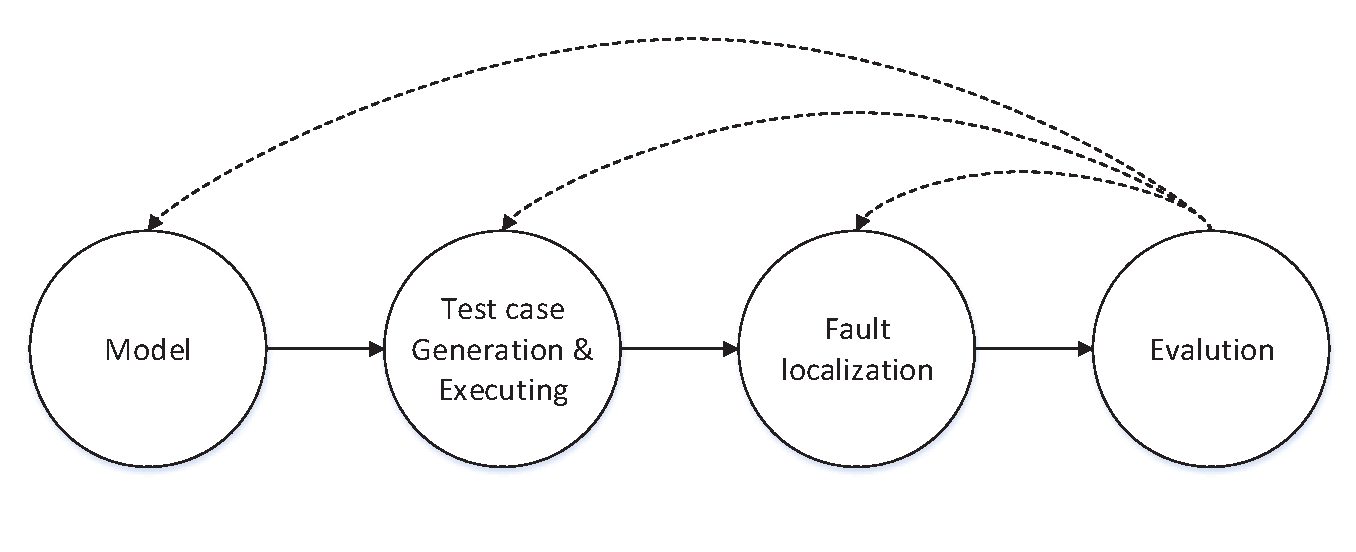
\includegraphics[width=3.4in]{CT_lifecircle.eps}
\caption{The life cycle of CT}
\label{ct-life}
\end{figure}




\section{Background}
This section presents some definitions and propositions to give a formal model for CT.

%\subsection{Failure-inducing interactions in CT}

Assume that the SUT is influenced by \emph{n} parameters, and each parameter $p_{i}$ can take the values from the finite set $V_{i}$ ($i$ = 1,2,..n). The definitions below are originally defined in \cite{nie2011minimal}.

\newdef{definition}{Definition}
\begin{definition}
A \emph{test case} of the SUT is a tuple of \emph{n} values, one for each parameter of the SUT. It is denoted as  ($v_{1}$, $v_{2}$,...,$v_{n}$), where $v_{1}\in V_{1}$, $v_{2} \in V_{2}$ ... $v_{n} \in V_{n}$.
\end{definition}
%a \emph{n}-tuple

In practice, these parameters in the test case can represent many factors, such as input variables, run-time options, building options or various combination of them. We need to execute the SUT with these test cases to ensure the correctness of the behaviour of the SUT.

%\begin{definition}
We consider any abnormally executing test case as a \emph{fault}. It can be a thrown exception, compilation error, assertion failure or constraint violation. When faults are triggered by some test cases, it is desired to figure out the cause of these faults. Some subsets of these test cases should be analysed.
%\end{definition}


\begin{definition}
For the SUT, the \emph{n}-tuple (-,$v_{n_{1}}$,...,$v_{n_{k}}$,...)is called a \emph{k}-degree \emph{schema} ($0 < k \leq n $) when some k parameters have fixed values and other irrelevant parameters are represented as "-".

In effect a test case itself is a k-degree \emph{schema}, when k = n. Furthermore, if a test case contains a \emph{schema}, i.e., every fixed value in the schema is in this test case, we say this test case \emph{contains} the \emph{schema}.
%, which can be denoted as $k-value\  combination \in T$
\end{definition}
Note that the schema is a formal description of the interaction between parameter values we discussed before.

\begin{definition}
Let $c_{l}$ be a \emph{l}-degree schema, $c_{m}$ be an \emph{m}-degree schema in SUT and $l < m$. If all the fixed parameter values in $c_{l}$ are also in $c_{m}$, then $c_{m}$ \emph{subsumes} $c_{l}$. In this case we can also say that $c_{l}$ is a \emph{sub-schema} of $c_{m}$ and $c_{m}$ is a \emph{super-schema} of $c_{l}$, which can be denoted as $c_{l} \prec  c_{m}$.
\end{definition}

For example,  the 2-degree schema (-, 4, 4, -) is a sub-schema of the 3-degree schema (-, 4, 4, 5), that is, (-,4,4,-) $\prec$ (-,4,4,5).

\begin{definition}
If all test cases that contain a schema, say $c$, trigger a particular fault, say $F$, then we call this schema $c$ the \emph{faulty schema} for $F$. Additionally, if none of sub-schema of $c$ is the \emph{faulty schema} for $F$, we then call the schema $c$ the \emph{minimal failure-causing schema (MFS)} \cite{nie2011minimal} for $F$.

%Based on this, if a test case $t$ hit such a failure-inducing combination, say $c(F)$, it should trigger the fault $F$, for which the test case can be put as $t(F)$
\end{definition}

Note that MFS is identical to the failure-inducing interaction we discussed previously. In this paper, the terms \emph{failure-inducing interactions} and \emph{MFS} are used interchangeably. Figuring the MFS out helps to identify the root cause of a failure and thus facilitate the debugging process.

\subsection{CT Test Case Generation}
When applying CT, the most important work is to determine whether the SUT suffers from the interaction faults or not, i.e., to  detect the existence of the MFS. Rather than impractically executing exhaustive test cases, CT commonly design a relatively small set of test cases to cover all the schemas with the degree no more than a prior fixed number, $t$. Such a set of test cases is called the \emph{covering array}.  If some test cases in the covering array failed in execution, then the interaction faults is regard to be detected.

Many studies in CT focus on how to generate such a test suite with the aim of making the size of the test suite as small as possible. In general, most of these studies can be classified into three categories according to the construction strategy of the covering array:

1) One test case one time : This strategy repeats generating one test case as one row of the covering array and counting the covered schemas achieved until all schemas are covered.

%  generate a completed test case to cover

2) A  set of test cases one time:  This strategy generates a set of test cases at each iteration. Through mutating the values of some parameters of some test cases in this test set, it focuses optimising the coverage. If the coverage is finally satisfied, it will reduce the size of the set to see if fewer test cases can still fulfil the coverage. Otherwise, it will increase the size of test set to cover all the schemas\cite{cohen2003augmenting}.

3) Others :  This strategy differentiates from the previous two strategies in that it does not firstly generate complete test cases \cite{lei2008ipog}. Instead, it first focuses on assigning values to some part of the factors or parameters to cover the schemas that related to these factors, and then fills up the remaining part to form complete test cases.

In this paper, we focus on the first strategy: One test case one time as it immediately get a complete test case such that the testers can execute and diagnose in the early stage. As we will see later, with respect to the MFS identification, this strategy is the most flexible and efficient one comparing with the other two strategies.

%To isolate the failure-inducing schemas and further bug fixing, the first step, is to detect them. To efficiently isolate the failure-inducing schemas, and to . Such a testing object, is covering array, which ,. Formally,
%
%\begin{definition}
%Covering array.
%\end{definition}

%Such a covering can , how to generate such a covering lying two facts.
%There are three different kinds of generation
%
%Overall test
%
%one test one time
%
%other special testing object.

%In order to fulfil the testing target, we choose the second object, one test one time, as we can .

\subsection{Identify the failure-inducing interactions}
To detect the existence of MFS in the SUT is still far from figuring out the root cause of the failure, as we do not know exactly which schemas in the failed test cases should be responsible for the failure. In fact, for a failing test case ($v_{1},v_{2},...,v_{n}$), there can be at most $2^{n} - 1$ possible schemas for the MFS. Hence, more test cases should be generated to identify the MFS. In CT, the main work in fault localization is to identify the failure-inducing interactions. So in this paper we only focus on the MFS identification. Further works of fault localization such as isolating the defect inside the source code will not be discussed.

A typical MFS identification process is shown in Table \ref{ofot-identify}. This example assumes the SUT has 3 parameters, each can take 2 values, and the test case (1, 1, 1) fails. Then in Table \ref{ofot-identify}, as test case \emph{t} failed, we mutate one factor of the \emph{t} one time to generate new test cases: $t_{1}$ -- $t_{3}$, It turns out that test case $t_{1}$ passed, which indicates that this test case break the MFS in the original test case \emph{t}. So (1,-,-) should be a failure-causing factor, and as other mutating process all failed, which means no other failure-inducing factors were broken, therefore, the MFS in \emph{t} is (1,-,-).

\begin{table}[h]
\caption{OFOT with our strategy}
\label{ofot-identify}
\center
\begin{tabular}{llllll}
 \hline
\multicolumn{5}{c}{\bfseries Original test case} & \bfseries Outcome \\  \hline
 $t$ & \multicolumn{4}{l}{1 \ \ \ \ 1 \ \ \ \  1 } & Fail \\
 \hline
\multicolumn{5}{c}{\bfseries Additional  test cases} &  \\  \hline
$t_{1}$ &\multicolumn{4}{l}{0  \ \ \ \  1 \ \ \ \  1 }& Pass \\
$t_{2}$ &\multicolumn{4}{l}{1  \ \ \ \  0 \ \ \ \  1 } & Fail \\
$t_{3}$ &\multicolumn{4}{l}{1  \ \ \ \  1 \ \ \ \  0 } & Fail \\
 \hline
\end{tabular}
\end{table}

This identification process mutate one factor of the original test case at a time to generate extra test cases. And then according to the outcome of the test cases execution result, it will identify the MFS of the original failing test cases. It is called the OFOT method, which is a well-known MFS identification method in CT. In this paper, we will focus on this identification method. It should be noted that the following proposed CT framework can be easily applied to other MFS identification methods.


\section{Motivating example}
%This section presents the .
%As discussed previously, the generation and identification are the most important stages in CT life-cycle. How to enhance these two activities in the CT life-cycle is of importance as it greatly impacts on the quality and cost of overall software testing. In fact, most studies in CT focus on these two fields. But rather than as a whole, generation and identification are applied independently. The justification for not discussing how to cooperate these two activities is that the first-generation-then-identification is so natural and straightforward. As we will show below, however, that the generation and identification is so tightly correlated that they have a significant impact on the effectiveness and efficiencies of testing.

A typical traditional generation-identification life-cycle is to first generate a $t$-way covering array. If there exists some failures that triggered by some particular schemas, then we detect some failures and should identify the MFS in the SUT for further bug fixing.

As an example, Table \ref{tradition-gi} illustrates the process of traditional CT. The SUT has 4 parameters and each parameter has three values. Traditional CT first generated and executed the 2-way covering array ($t_{1}$ -- $t_{9}$). Note that this covering array covered all the 2-degree schemas for the SUT. And after finding that $t_{1}$, $t_{2}$, and $t_{7}$ failed during testing, it then respectively identified the MFS in $t_{1}$ ,$t_{2}$, and $t_{7}$. For $t_{1}$, it used the OFOT method to generate four additional test cases ($t_{10}$ -- $t_{13}$), and identified the MFS of $t_{1}$ is (-, 0, - , -) as only when changing the second factor of $t_{1}$ it will pass. Then it applied the same process to $t_{2}$ and $t_{7}$, and found that (-,0, -, -) is also the MFS of $t_{2}$ and $t_{7}$.  Finally, for detecting and identifying the MFS in this example SUT, we have generated 12 additional test cases(marked with star).
%It must be noted that, when isolating the MFS of $t_{2}$, the generated extra test cases $t_{9}$ and $t_{10}$ has appeared before, so we can just reuse the previous result.

\begin{table}[h]
\caption{Traditional generation-identification life-cycle}
\label{tradition-gi}
\center
\begin{tabular}{llllll}
\hline
\multicolumn{6}{c}{\bfseries \emph{Generation}} \\
\hline
\multicolumn{5}{c}{\bfseries test case} & \bfseries Outcome \\
 $t_{1}$ & \multicolumn{4}{l}{0 \ \ \ \ 0 \ \ \ \  0\ \ \ \ 0} & Fail \\
 $t_{2}$ & \multicolumn{4}{l}{0 \ \ \ \ 1 \ \ \ \  1\ \ \ \ 1} & Pass \\
 $t_{3}$ & \multicolumn{4}{l}{0 \ \ \ \ 2 \ \ \ \  2\ \ \ \ 2} & Pass \\
 $t_{4}$ & \multicolumn{4}{l}{1 \ \ \ \ 0 \ \ \ \  1\ \ \ \ 2} & Fail \\
 $t_{5}$ & \multicolumn{4}{l}{1 \ \ \ \ 1 \ \ \ \  2\ \ \ \ 0} & Pass \\
 $t_{6}$ & \multicolumn{4}{l}{1 \ \ \ \ 2 \ \ \ \  0\ \ \ \ 1} & Pass \\
 $t_{7}$ & \multicolumn{4}{l}{2 \ \ \ \ 0 \ \ \ \  2\ \ \ \ 1} & Fail \\
 $t_{8}$ & \multicolumn{4}{l}{2 \ \ \ \ 1 \ \ \ \  0\ \ \ \ 2} & Pass \\
 $t_{9}$ & \multicolumn{4}{l}{2 \ \ \ \ 2 \ \ \ \  1\ \ \ \ 0} & Pass \\
 \hline
\multicolumn{6}{c}{\bfseries \emph{Identification}}  \\
\hline
\multicolumn{5}{c}{\bfseries for $t1$--- 0 0 0 0} &  \\
$t_{10}$* &\multicolumn{4}{l}{1  \ \ \ \  0 \ \ \ \  0 \ \ \ \  0} & Fail \\
$t_{11}$* &\multicolumn{4}{l}{0  \ \ \ \  1 \ \ \ \  0 \ \ \ \  0} & Pass \\
$t_{12}$* &\multicolumn{4}{l}{0  \ \ \ \  0 \ \ \ \  1  \ \ \ \ 0} & Fail \\
$t_{13}$* &\multicolumn{4}{l}{0  \ \ \ \  0 \ \ \ \  0  \ \ \ \ 1} & Fail \\
\multicolumn{6}{c}{\bfseries result --  (-, 0, -, -)}  \\
\multicolumn{5}{c}{\bfseries for $t4$--- 1 0 1 2} &  \\
$t_{14}$* &\multicolumn{4}{l}{2  \ \ \ \  0 \ \ \ \  1 \ \ \ \  2} & Fail \\
$t_{15}$* &\multicolumn{4}{l}{1  \ \ \ \  1 \ \ \ \  1 \ \ \ \  2} & Pass \\
$t_{16}$* &\multicolumn{4}{l}{1  \ \ \ \  0 \ \ \ \  2  \ \ \ \ 2} & Fail \\
$t_{17}$* &\multicolumn{4}{l}{1  \ \ \ \  0 \ \ \ \  1  \ \ \ \ 0} & Fail \\
\multicolumn{6}{c}{\bfseries result --  (-, 0, -, -)}  \\
\multicolumn{5}{c}{\bfseries for $t7$--- 2 0 2 1} &  \\
$t_{18}$* &\multicolumn{4}{l}{0  \ \ \ \  0 \ \ \ \  2 \ \ \ \  1} & Fail \\
$t_{19}$* &\multicolumn{4}{l}{2  \ \ \ \  1 \ \ \ \  2 \ \ \ \  1} & Pass \\
$t_{20}$* &\multicolumn{4}{l}{2  \ \ \ \  0 \ \ \ \  0  \ \ \ \ 1} & Fail \\
$t_{21}$* &\multicolumn{4}{l}{2  \ \ \ \  0 \ \ \ \  2  \ \ \ \ 2} & Fail \\
\multicolumn{6}{c}{\bfseries result --  (-, 0, -, -)}  \\
\hline
\end{tabular}
\end{table}

We refer to such traditional life-cycle as \emph{\textbf{sequential CT}}. However, we believe this may not be the best choice in practice. The first reason is that the engineers normally do not want to wait for fault localization after all the test cases are executed. The early bug fixing is appealing and can give the engineers confidence to keep on improving the quality of the software. The second reason, which is also the most important, is such life-cycle can generate many redundant and unnecessary test cases. This can be reflected in the following two aspects:

1) The test cases generated in the identification stage can also contribute some coverage, i.e., the schemas appear in the passing test cases in the identification stage may have already been covered in the test cases generation stage.  For example, when we identify the MFS of $t_{1}$ in Table \ref{tradition-gi}, the schema (0, 1, -, -) contained in the extra passing test case $t_{11}$ -- (0, 1, 0, 0) has already been appeared in the passing test case $t_{2}$ -- (0, 1, 1, 1). In other word, if we firstly identify the MFS of $t_{1}$, then $t_{2}$ is not a good choice as it does not covered as many 2-degree schemas as possible. For example, (1, 1, 1, 1) is better than this test case at contributing more coverage.

2)The identified MFS should not appear in the following generated test cases.  This is because according to the definition of MFS, each test case containing this schema will trigger a failure, i.e., to generate and execute more than one test case contained the MFS makes no sense for the failure detecting. Even worse, such test case may suffer from the \emph{masking effects} \cite{yilmaz2013reducing}, as failures caused by the already identified MFS can prevent the test case from normally checked (e.g., failures that can trigger an unexpected halt of the execution). As a result, some schemas in these test cases that are supposed to be examined will actually skip the testing. Take the example in Table \ref{tradition-gi}, after identifying the MFS -- (-, 0, -, -) of $t_{1}$, we should not generate the test case $t_{4}$ and $t_{7}$. This is because they also contain the identified MFS (-, 0, -, -), which will result in them failing as expected. Surely the expected failure caused by MFS (-, 0, -, -) makes $t_{4}$ and $t_{7}$ superfluous for error-detection, and even worse some other schemas in $t_{4}$ or $t_{7}$  may be masked, as those schemas can potentially trigger other failures but will not be observed. And since we should not generate $t_{4}$ and $t_{7}$,  the additional test cases ($t_{14}$ to $t_{21}$)generated for identifying the MFS in $t_{4}$ and $t_{7}$ are also not necessary.

Based on these observations, a more effective and efficient framework is desired.

\section{Traditional approach limitation}
\subsection{reduntant test cases}

\subsection{mulitple MFS in one test case}
non overlap

overlap


\subsection{masking effects}


\section{empirically study}

\subsection{software subjects}

\subsection{compare with traditional test cases}

test cases

redundant test cases (generate and identify)


\subsection{multiple MFS}

multiple failures in one test case

f-measure

overlap and non overallp





\subsection{masking effects}
masking effects condition.




integrated. using FDA-CIT to make it adequte testing



\section{Limitations of our approach}
\subsection{incorrect schemas}
incorrect schemas can give us unrelieble results. However, this is inavoid. To definely get exact MFS, according to charle courblun and Nie , we need to exhaustive condunct every possible test cases, which is however, not possible. So in practice, we get an ���ƽ� [Zeller's paper to show how global minimal is not possible].

Based on this, if our algorithm get an wrong MFS, then it can be .


\emph{Possible solution}
1) Multiple approaches combined, this will enhance the ³���� of our method. As we can learn in the emprically study, the combination of FDA-CI can significantly improve the prisce of the MFS identification and testing adquattely.

2) More critically feedback validation. That is, when a MFS is identified. We need to send to the developers to see whether it is one of the root cause of failure. And if correct, then we go on. Else, we will re-compute the MFS with the developers information.




\subsection{constraints handling}

As to avoid the idenified MFS is needed. In this paper, we handle this as constraints, which needs to get an solver to aviod the following result. This handling, however, obviously increase the cost of the whole CT process. As constraints satification (SAT) problem and optimcal problem (covering array) is both tough [][][][][], the increasing is possible.

\emph{Possible solution}

1) Illustrate history to reducation

2) better practical stop [Zeller' paper saied a good term, to show why isolation)

3) better constratins modeling


\section{Interleaving Approach}

To overcome such deficiencies in traditional CT, we propose a new CT generation-identification framework -- \emph{\textbf{Interleaving CT}}. Our new framework aims at enhancing the interaction of generation and identification to reduce the unnecessary and invalid test cases discussed previously.


\subsection{Overall framework}
 The basic outline of our framework is illustrated in Figure \ref{new-life}.
\begin{figure}
 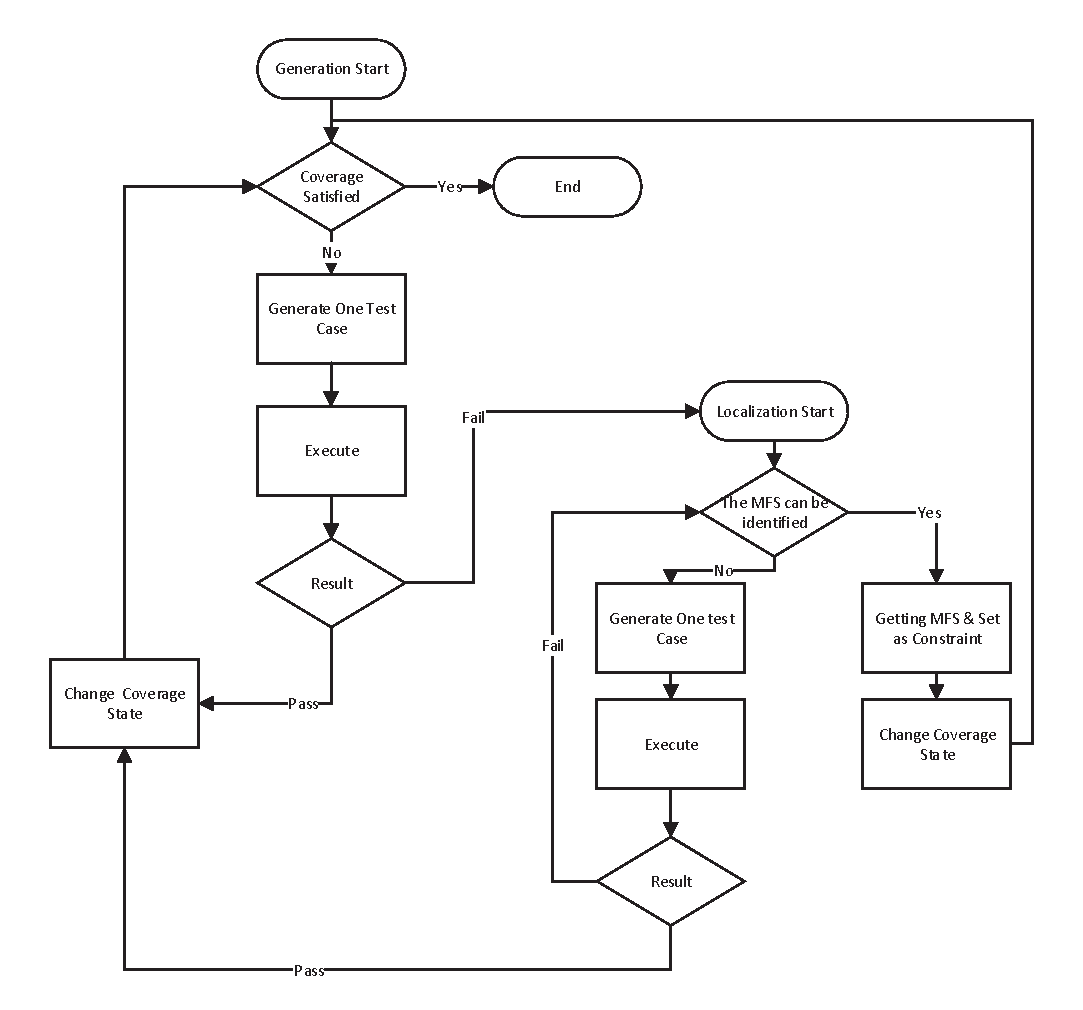
\includegraphics[width=3.4in]{baicOutline.eps}
\caption{The Interleaving Framework}
\label{new-life}
\end{figure}
Specifically, this new framework works as follows: First, it checks whether all the needed schemas are covered or not. Commonly the target of CT is to cover all the $t$-degree schemas, with $t$ normally be assigned as 2 or 3. Then if the current coverage is not satisfied, it will generate a new test case to cover as many uncovered schemas as possible. After that, it will execute this test case with the outcome of the execution either be pass (executed normally, i.e., does not triggered an exception, violate the expected oracle or the like) or fail (on the contrary). When the test case passes the execution, we will recompute the coverage state, as all the schemas in the passing test case are regarded as error-irrelevant. As a result, the schemas that was not covered before will be determined to be covered if it is contained in this newly generated test case. Otherwise if the test case fails, then we will start the MFS identification module to identify the MFS in this failing test case. One point that needs to be noted is that if the test case fails, we will not directly change the coverage, as we can not figure out which schemas are responsible for this failure among all the schemas in this test case until we identify them.

The identification module works in a similar way as traditional independent MFS identify process, i.e., repeats generating and executing additional test cases until it can get enough information to diagnose the MFS in the original failing test case. The difference from traditional MFS identifying process is that we record the coverage that this module has contributed to the overall coverage. In detail, when the additional test case passes, we will label the schemas in these test cases as covered if it has not been covered before. And when the MFS is found at the end of this module, we will first set them as forbidden schemas that latter generated test cases should not contain (Otherwise the test case must fail and it cannot contribute to more coverage), and second all the $t$-degree schemas that are \emph{related} to these MFS as covered. Here the \emph{related} schemas indicate the following three types of $t$-degree schemas:

First, the MFS \textbf{themselves}. Note that we do not change the coverage state after the generated test case fails (both for the generation and identification module ), so these MFS will never be covered as they always appear in these failing test cases.

Second, the schemas that are the \textbf{super-schemas} of these MFS. By definition of the super-schemas (Definition 3), if the test case contains the super-schemas, it must also contain all its sub-schemas. So every test case that contains the super-schemas of the MFS must fail after execution. As a result, they will never be covered as we do not change the coverage state for failing test cases.

Third, those \textbf{implicit forbidden} schemas, which was first introduced in \cite{cohen2007interaction}.  This type of schemas are caused by the conjunction of multiple MFS. For example, for a SUT with three parameters, and each parameter has two values, i.e., SUT(2, 2, 2). If there are two MFS for this SUT, which are (1, -, 1) and (0, 1, -). Then the schema (-, 1, 1) is the implicit forbidden schema. This is because for any test case that contain this schema, it must contain either (1, -, 1) or (0, 1, -). As a result, (-, 1, 1) will never be covered as all the test cases containing this schema will fail and so we will not change the coverage state. In fact, by Definition 4, they can be deemed as faulty schemas.

As we all know, the terminating condition of the CT framework is to cover all the $t$-degree schemas. Then since the three types of schemas will never be covered in our new CT framework, we can set them as covered after the execution of the identification module, so that the overall process can stop.

\subsection{Modifications of CT activities}
More details of the modifications of CT activities are as follows:

(1) \emph{Modified CT Generation} :
We adopt the \emph{one test case one time} method as the basic skeleton of the generation process. Originally, the generation of one test case can be formulated as \ref{eq1}.
\begin{displaymath} t \leftarrow  select (\mathcal{T}_{all}, \Omega ,  \xi) \tag{EQ1} \label{eq1} \end{displaymath}

There are three factors that determine the selection of test case $t$. $\mathcal{T}_{all}$ represents all the valid test cases that can be selected to be executed. Usually the test cases that have been tested will not be included as they have no more contribution to the coverage. $\Omega$ indicates the set of schemas that have not been covered yet. $\xi$ is a random factor. Most CT generation approaches prefer to select a test case that can cover as many uncovered schemas as possible. This greedy selection process does not guarantee an optimal solution, i.e., the final size of the set of test cases is not guaranteed to be minimal. The random factor $\xi$ is used to help to escape from local optimum.

%the parameters and their values, which indicates a valid test case. $\Omega$ gives the uncovered schemas currently. Note that the is to . To the oppiste , each test case. It is noted that for a . Thus some random factor $xi$ is needed to the local optimization.


As discussed in section 3, we should make the MFS not appear in the test cases generated afterwards, by treating them as the forbidden schemas. In other words, the candidate test cases that can be selected are reduced, because those test cases that contain the currently identified MFS should not appear next. Formally,  let $\mathcal{T}_{MFS}$ indicates the set of test cases that contain the currently identified MFS, then the test case selection is augmented as \ref{eq2}.
\begin{displaymath} t \leftarrow  select (\mathcal{T}_{all} - \mathcal{T}_{MFS}, \Omega ,  \xi ) \tag{EQ2} \label{eq2} \end{displaymath}

In this formula, the only difference from \ref{eq1} is that the candidate test cases that can be selected are changed to $\mathcal{T}_{all} - \mathcal{T}_{MFS}$, which excludes $\mathcal{T}_{MFS}$ from candidate test cases.

In practice, it is impossible to thoroughly search the exhaustive candidate test cases $\mathcal{T}_{all}$ to get a specific test case $t$. Hence, some heuristic methods are used to simplify the selection. For example, AETG \cite{cohen1997aetg} successively assigns the value to each parameter to form a test case (in random order). The value to be assigned is the one that appears in the greatest number of uncovered schemas. Correspondingly, to exclude the test cases in $\mathcal{T}_{MFS}$, it is common to utilize a constraint solver to avoid the forbidden schemas \cite{cohen2007interaction,cohen2008constructing}.

%Our test case generation with consideration for constraints is inspired by the  based on which we give an more general approach that can be applied on more one-test-one-time generation methods.  The detail of how to generate one test case is described in Algorithm 1.


%
%
%This will transfer to the




%$\mathcal{M}$ indicates the MFS that are currently identified. And should not be contained.


(2) \emph{Modified identification of MFS} : Traditional MFS identification aims at finding the MFS in a failing test case. As discussed before, test cases in the covering array are not enough to identify the MFS. Hence, additional test cases should be generated and executed in this CT activity. Generally, an additional test case is generated based on the original failing test case, so that the failure-inducing parts can be determined by comparing the difference between the additional test cases and the original failing test cases. Take the OFOT approach as an example. In Table \ref{tradition-gi}, the additional test case $t_{11}$ is constructed by mutating the second parameter value of the original failing test case $t_{1}$. Then as $t_{11}$ passed the testing, we can determine that the second parameter value (-, 0, -, -) must be a failure-inducing element. Formally, let $t_{failing}$ be the original failing test case, $\Delta$ be the mutation parts, $\mathcal{P}$ be the parameters and their values, then the traditional additional test case generation can be formulated as \ref{eq3}.
\begin{displaymath}t \leftarrow  mutate (\mathcal{P}, t_{failing}, \Delta )  \tag{EQ3} \label{eq3} \end{displaymath}

\ref{eq3} indicates that the test case $t$ is generated by mutating the part $\Delta$ of the original failing test case $t_{failing}$. Note that the mutated values may have many choices, as long as they are within the scope of $\mathcal{P}$ and different from those in $t_{failing}$. For example, for the original failing test case $t_{1}$ (0,0,0,0) in Table \ref{tradition-gi}, let $\Delta$ be the second parameter value, then test cases (0, 1, 0, 0) and (0, 2, 0, 0) all satisfy \ref{eq3}. We refer to all the test cases that satisfy \ref{eq3} as $\mathcal{T}_{candidate}$, which can be formulated  as   \ref{eq4}.
\begin{displaymath}\mathcal{T}_{candidate} =  \{\ t\ |\ t \leftarrow  mutate (\mathcal{P}, t_{failing}, \Delta )\ \} \tag{EQ4} \label{eq4} \end{displaymath}
Traditional MFS identification process just selects one test case from $\mathcal{T}_{candidate}$ randomly. However, to adapt the MFS identification process to the new CT framework, this selection should be refined.

%let $\mathcal{T}_{candidate}$ be  the initial candidate test cases as \ref{eq4}. This set collects all the possible test cases by mutating the the part $\Delta$ of the original test case $t_{failing}$.
Specifically, there are two points to note. First, the additional test case should not contain the currently identified MFS; second, the additional test case is expected to cover as many uncovered schemas as possible. These two goals are similar to CT generation, hence we can directly apply the same selection method on additional test case generation, which can be formulated as \ref{eq5}.  The same as \ref{eq2}, \ref{eq5} excludes the test cases that contain the currently identified MFS from the candidate test cases ($\mathcal{T}_{candidate} - \mathcal{T}_{MFS}$), and selects the additional test case which covers the greatest number of uncovered schemas ($\Omega$).
\begin{displaymath}t \leftarrow  select (\mathcal{T}_{candidate} - \mathcal{T}_{MFS}, \Omega ,  \xi )  \tag{EQ5} \label{eq5} \end{displaymath}


%The identification process should also . From Figure \ref{new-life}, we can find some part of this process to identify the MFS is similar to that of the $generation$

%module, i.e., they all need to repeat generating test cases until reach some criteria. As for the additional test cases generated in the identification process, Based on the two points, the additional test cases generation in the CT identification should be refined as in Algorithm 2.


%We can observe that this algorithm is very similar to Algorithm 1, except that this algorithm introduce the variables $ f_{original}$ and $s_{fixed}$. These two variables are important to MFS identification. Generally, the target of the MFS identification process is to distinguish the MFS from those error-irrelevant schemas in a failing test case. For this, the MFS identification process need to generate and execute additional test cases to compare to original failing test case $f_{original}$. The additional test case must contain some fixed schema $s_{fixed}$ in the $f_{original}$, and other part of the additional test case must be different from $f_{original}$ (line 4).  By doing this, this identification process can check whether the $fixed$ are failure-inducing or not. For example, in Table \ref{ofot-identify}, the original failing test case is (1, 1, 1 ) and the fixed part for additional test case $t_{1}$ (0, 1, 1) is (-, 1, 1). After the $t_{1}$ passed during testing, we can get that the fixed schema (-, 1, 1) should not be the MFS.
%
%Traditional MFS identification process just need to ensure that the $mutant$ part have different values from original failing test cases. We augmented this by selecting values that can cover as more uncovered schemas as possible (line 6) and to ensure the test case does not contain some identified MFS (line 7 - 8).

(3) \emph{Updating uncovered schemas} :
After the MFS are identified, some related $t$-degree schemas, i.e., \emph{MFS themselves}, \emph{super-schemas} and \emph{implicit forbidden schemas}, should be set as covered to enable the termination of the overall CT process. The algorithm that seeks to handle these three types of schemas is listed in Algorithm 1.


\begin{algorithm}
  \caption{Changing coverage after identification of MFS}
  \begin{algorithmic}[1]
     \Require

    % $t_{original}$ \Comment{original failing test case}


     $\mathcal{S}_{MFS}$ \Comment{currently identified MFS}

     $\Omega$ \Comment{the schemas that are still uncovered}


     $\mathcal{T}_{all}$ \Comment{all the possible test cases}

     $\mathcal{T}_{MFS}$ \Comment{all the test cases that contain the MFS}

\Ensure  $void$ \Comment{do not need any output}
\
   %  \ForAll  {$s \in S_{identified}$}
%       \State $S_{MFS}.append(s)$
%     \EndFor
     \ForAll {$s  \in  \mathcal{S}_{MFS}$}
       \If {$s$\ is\ $t$-degree\ schema}
          \State $\Omega \leftarrow \Omega \backslash s$
       \EndIf
       \ForAll {$s_{p}$\ is\ super-schema\ of\ $s$}
         \If {$s_{p}$\ is\ $t$-degree\ schema}
          \State $\Omega \leftarrow \Omega \backslash s_{p}$
         \EndIf
       \EndFor
     \EndFor
     \ForAll {$s \in \Omega$}
       \If {$\not\exists t \in (\mathcal{T}_{all} - \mathcal{T}_{MFS}), s.t., t.contain(s)$}
         \State  $\Omega \leftarrow \Omega \backslash s$
       \EndIf
     \EndFor
  \end{algorithmic}
\end{algorithm}

 In this algorithm, we firstly check each MFS (line 1) to see if it is $t$-degree schema (line 2). We will set those $t$-degree MFS as covered and remove them from the uncovered schemas set $\Omega$ (line 3). This is the first type of schemas --\emph{themselves}. For each $t$-degree super-schema of these MFS, it will also be removed from the uncovered schemas set (line 5 - 9), as they are the second type of schemas --  \emph{super-schemas}. The last type, i.e., \emph{implicit forbidden schemas}, is the toughest one. To remove them, we need to search through each potential schema in the uncovered schemas set (line 11), and check if it is the implicit forbidden schema (line 12). The checking process involves solving a satisfiability problem. Specifically, if we can not find a test case from  the set ($\mathcal{T}_{all} - \mathcal{T}_{MFS}$) (excluding those that contain MFS), such that it contains the schema under checking, then we can determine the schema is the implicit forbidden schema and it needs to be removed from uncovered schemas set (line 13). This is because in this case, the schema under checking can only appear in $\mathcal{T}_{MFS}$, which we will definitely not generate in later iterations. In this paper, a SAT solver will be utilized to do this checking process.

% Specifically, it checks whether the schema must exists with at least one . Then this schema will be set as \emph{implicit forbidden schemas} and set as covered.and the Constraints must be appeared in one
%
% Note that are executed each time a MFS is identified.
% This checking process is the same as we discussed in the Algorithm 1 and Algorithm 2.

% To find them from the uncovered set, we use a sat solver to
%he uncovetred  search through the uncovered schemas set (line 4), to eliminate these schemas that cannot avoid some MFS when extend these schemas into a test case(line 5 - 7).

%3) Setting constraint, and change coverage.



%Then the generation should not include, the characterization is should.

%To implement such framework, the most important is to share the information. In specific, to, we use the SAT solver. And when , we should change the coverage information. Our detail implementation for this framework is list in Algorithm.
\subsection{Example}

With this new framework, when we re-consider the example in Table \ref{tradition-gi} in section 3,  we can get the result listed in Table \ref{new-gi}.
\begin{table}[h]
\caption{Interleaving CT case study}
\label{new-gi}
\center
\begin{tabular}{llllll|llllll}
\hline
 & \multicolumn{4}{c}{\bfseries \emph{Generation}}& & \multicolumn{6}{c}{\bfseries \emph{Identification}} \\
 \hline
%\multicolumn{5}{c}{\bfseries test case} & \bfseries Outcome \\
$t_{1}$ & \multicolumn{4}{l}{0 \ \ \ 0 \ \ \ 0  \ \ \  0 } & Fail & \multicolumn{6}{l}{}\\
\multicolumn{5}{l}{}& & $t_{2}$* &\multicolumn{4}{l}{1  \ \ \  0 \ \ \  0 \ \ \  0 }& Fail \\
\multicolumn{5}{l}{}& &$t_{3}$* &\multicolumn{4}{l}{0  \ \ \   1 \ \ \  0 \ \ \  0} & Pass \\
\multicolumn{5}{l}{}& &$t_{4}$* &\multicolumn{4}{l}{0  \ \ \   0 \ \ \   1 \ \ \  0} & Fail \\
\multicolumn{5}{l}{}& &$t_{5}$* &\multicolumn{4}{l}{0  \ \ \   0 \ \ \   0 \ \ \   1} & Fail \\
\multicolumn{5}{l}{}& &\multicolumn{6}{l}{ \bfseries{MFS}: $(-, 0, - , -)$ }  \\
$t_{6}$ &\multicolumn{4}{l}{0 \ \ \ 1 \ \ \ 1  \ \ \  1 } & Pass & \multicolumn{6}{l}{}\\
$t_{7}$ &\multicolumn{4}{l}{0 \ \ \ 2 \ \ \ 2  \ \ \  2 } & Pass & \multicolumn{6}{l}{}\\
$t_{8}$ &\multicolumn{4}{l}{1  \ \ \ 1 \ \ \ 1  \ \ \  2 } & Pass & \multicolumn{6}{l}{}\\
$t_{9}$ &\multicolumn{4}{l}{1  \ \ \  1 \ \ \ 2 \ \ \ 0 } & Pass & \multicolumn{6}{l}{}\\
$t_{10}$ &\multicolumn{4}{l}{1  \ \ \   2 \ \ \   0 \ \ \ 1} & Pass & \multicolumn{6}{l}{}\\
$t_{11}$ &\multicolumn{4}{l}{2  \ \ \   1 \ \ \ 2  \ \ \  1 } & Pass & \multicolumn{6}{l}{}\\
$t_{12}$ &\multicolumn{4}{l}{2  \ \ \   1 \ \ \ 0  \ \ \  2 } & Pass & \multicolumn{6}{l}{}\\
$t_{13}$ &\multicolumn{4}{l}{2  \ \ \   2 \ \ \ 1  \ \ \  0 } & Pass & \multicolumn{6}{l}{}\\
\hline
\end{tabular}
\end{table}

This table consists of two main columns, in which the left indicates the generation part while the right column indicates the identification process. We can find that, after identifying the MFS (-, 0, -, -) for $t_{1}$, the following test cases ($t_{6}$ to $t_{13}$) will not contain this schema. Correspondingly, all the 2-degree schemas that are related to this schema, e.g. (0, 0, -, -), (-, 0, 1, -), etc, will also not appear in the following test cases. Additionally, the passing test case $t_{3}$ generated in the identification process cover six \emph{2}-degree schemas, i.e., (0, 1, -, -), (0, -, 0, -), (0, -, -, 0), (-, 1, 0, -), (-, 1, -, 0), and (-, -, 0, 0) respectively, so that it is not necessary to generate more test cases to cover them.  Above all, when using the interleaving CT approach,  the overall generated test case are 8 less than that of the traditional sequential CT approach in Table \ref{tradition-gi}.

Note that this example only lists the condition of a single MFS, under which some \emph{super-schemas} or \emph{themselves} will not need to be covered.  When there are multiple MFS, additional \emph{implicit forbidden} schemas will be computed and set as covered.

%Besides the cost reducing, our new CT framework actually provide a stronger coverage criteria than traditional covering array. This is because


%Up to now, all the 2-degree schemas are covered, in detail, (1  1 -) (1 - 1) (- 1 1) are covered by passing test case (1 1 1), (1 0 -) (1 - 0) (- 0 0) are covered by passing test case (1 0 0), (- 0 1) and (- 1 0) are covered by test case (1 0 1) and (1 1 0) respectively. Those schemas related to (0 - -) such as (0 - 1), (0 0 -) will not be covered as the (0 - -) is the MFS.  All the generated 7 test cases are not duplicated with each other (all marked *), we can find the overall generated test case are one less than the traditional approaches in Table \ref{tradition-gi}.
%\subsection{Description}
%
%
%\subsection{A case study}

\section{empirical studies}
To evaluate the effectiveness and efficiency of the interleaving CT approach, we conducted a series of empirical studies on several open-source software subjects.

\subsection{Subject programs}
The five subject programs used in our experiments are listed in Table \ref{subject}. Column ``Subjects" indicates the specific software. Column ``Version" indicates the specific version that is used in the following experiments. Column ``LOC" shows the number of source code lines for each software. Column ``Faults" presents the fault ID, which is used as the index to fetch the original fault description at each bug tracker for that software. Column ``Lan" shows the programming language for each software (For subjects written in more than one programming languages, only the main programming language is shown).

\begin{table}[ht]
\caption{Subject programs}
\label{subject}
\center
\begin{tabular}{l|l|l|l|l}
\hline
Subjects & Version & LOC & Faults &  Lan \\
\hline
Tomcat   &   7.0.40      & 296138    &   \#55905   & java  \\
Hsqldb   &   2.0rc8  &   139425   &    \#981     & Java \\
Gcc      &   4.7.2      &  2231564   & \#55459       &  c\\
Jflex    &    1.4.1     & 10040    &    \#87    & Java \\
Tcas     & $v_{1}$     &   173  &    \#Seed  & c \\ \hline
\end{tabular}

\end{table}

Among these subjects, Tomcat is a web server for java servlet; Hsqldb is a pure-java relational database engine; Gcc is a programming language compiler; Jflex is a lexical analyzer generator; and Tcas is a module of an aircraft collision avoidance system. We select these software as subjects because their behaviours are influenced by various combinations of configuration options or inputs. For example, one component \emph{connector} of Tomcat is influenced by more than 151 attributes \cite{tomcatconnector}. For program Tcas, although with a relatively small size (only 173 lines), it also has 12 parameters with their values ranged from 2 to 10. As a result, the overall input space for Tcas can reach 460800 \cite{shakya2012isolating,kuhn2006pseudo}.

As the target of our empirical studies is to compare the ability of fault defection between our approach with traditional ones, we firstly must know these faults and their corresponding MFS in prior, so that we can determine whether the schemas identified by those approaches are accurate or not.  For this, we looked through the bug tracker of each software and focused on the bugs which are caused by the interaction of configuration options. Then for each such bug, we derive its MFS by analysing the bug description report and the associated test file which can reproduce the bug. For Tcas, as it does not contain any fault for the original source file, we took an mutation version for that file with injected fault. The mutation was the same as that in \cite{kuhn2006pseudo}, which is used as a experimental object for the fault detection studies.

%To make the testing process can definitely find failing test cases (otherwise we may not detect any fault and then there is no difference between our approach with traditional approach), we prepared fault version of these software in prior. There are four software, we take the real failures, for each failure, there bug tracker can be find .  The last one is the injected failure, which is originally injected in .


\subsubsection{Specific inputs models}
To apply CT on the selected software, we need to firstly model their input parameters. As we discussed before, the whole configuration options is extremely large so that we cannot include all of them in our model in consideration of the experimental time and computing resource. Instead, a moderate small set of these configuration options is selected.  It includes the options that cause the specific faults in Table \ref{subject}, thus the test cases generated by CT can detect these faults. Additional options are also included to create some noise for the MFS identification approach. These options are selected randomly. Details of the specific options and their corresponding values of each software are posted at \texttt{http://barbie.uta.edu/data.htm}.  A brief overview of the inputs models as well as the corresponding MFS (degree) is shown in Table \ref{inputs}.

%As our study is focus on combinatorial testing,
% we must take the faults,  Some faults we collected are it. To let our CT model more applied. We add some additional options that can happen interactive events to them. We let them . To get the real MFS, note that the additional , we need to exhaustive execute all the test cases, so that we limited them at a moderate level.

\begin{table}[ht]
\caption{Inputs model }
\label{inputs}
\center
\begin{tabular}{l|l|l}
\hline
Subjects & Inputs & MFS \\
\hline
Tomcat   &  $2^{8} \times 3^{1} \times 4^{1}$       & 1(1) 2(2)  \\
Hsqldb   &   $2^{9} \times 3^{2} \times 4^{1}$      &  3(2) \\
Gcc      &   $2^{9} \times 6^{1}$      &    3(4)  \\
Jflex    & $2^{10} \times 3^{2} \times 4^{1} $        &   2(1)   \\
Tcas     &  $2^{7} \times 3^{2} \times 4^{1} \times 10^{2} $ &9(16)\ 10(8)\ 11(16)\ 12(8) \\ \hline
\end{tabular}

\end{table}
In this table, Column ``inputs" depicts the input model for each version of the software, presented in the abbreviated form $\#values^{\#number\ of\ parameters} \times ...$, e.g., $2^{9} \times 3^{2} \times 4^{1}$ indicates the software has 9 parameters that can take 2 values, 2 parameters can take 3 values, and only one parameter that can take 4 values. Column ``MFS" shows the degrees of each MFS and the number of MFS (in the parentheses) with that corresponding degree.

\subsection{Comparing with sequential CT}

After preparing the subjects software, next we constructed the experiment to evaluate the efficiency and effectiveness of our approach. To this aim, we need to compare our framework with the traditional sequential CT approach to see if interleaving CT approach has any advantage.

The covering array generating algorithm used in the experiment is AETG \cite{cohen1997aetg}, as it is the most common one-test-case-one-time generation algorithm. And the MFS identifying algorithm is OFOT \cite{nie2011minimal} as discussed before. The constraints handling solver is a java SAT solver -- SAT4j \cite{le2010sat4j}.


\subsubsection{Study setup}
For each software except \emph{Tcas}, a test case is determined to be passing if it ran without any exceptions; otherwise it is regarded as failing. For \emph{Tcas}, as the fault is injected, we determine the result of a test case by separately running it with the original correct version and the mutation version. The test case will be labeled as passing if their results are the same; otherwise, it is deemed as failing.

In this experiment, we focus on three coverage criteria, i.e., 2-way , 3-way and 4-way, respectively. It is known that the generated test cases vary for different runs of AETG algorithm. So to avoid the biases of randomness, we conduct each experiment 30 times and then evaluate the results.  In other word, for each subject software, we will repeatedly execute traditional approach and our approach 30 times to detect and identify the MFS.
% For each %run of the experiment, we respectively set the coverage criteria, 2-way, 3-way and 4-way.

To evaluate the results of the two approaches, one metric is the cost, i.e., the number of test cases that each approach needs. Specifically, the test cases that are generated in the CT generation and MFS identification, respectively, are recorded and compared for these two approaches.  Apart from this, another important metric is the quality of their identified MFS. For this, we used standard metrics: \emph{precision} and \emph{recall}, which are defined as follows:

$$precision =  \frac{\#the\ num\ of\ correctly\ identified\  MFS}{\#the\ num\ of\ all\ the\ identified\ schemas}$$
and
$$recall  =  \frac{\#the\ num\ of\ correctly\ identified\  MFS}{\#the\ num\ of\ all\ the\ real\ MFS} $$

\emph{Precision} shows the degree of accuracy of the identified schemas when comparing to the real MFS. \emph{Recall} measures how well the real MFS are detected and identified. The combination of them is F-measure, which is
$$F-measure = \frac{2 \times precision \times recall}{precision + recall}$$
%
%There are two metrics we care in this experiment. First, the overall test cases that each approach needed. This metric indicates the cost that each approach will take. Second, the quality of the identified MFS, i.e., how accurately the schema each approach identified when compared with the real MFS we figured out in prior.  To assess this metric, we define the similarity between two schemas as follows:
%
%\begin{displaymath} Similarity(S_{A},S_{B})= \frac{the\ same\ elements\ in\ S_{A}\ and\ S_{B}}{\max (Degree(S_{A}),Degree(S_{B})) } \end{displaymath}.
%
%The numerator of this formula shows the same elements of two schemas ($S_{A}$ and $S_{B}$), and the denominator normalizes the overall metric.  For example, the similarity of  (- 1\ 2 - 3) and  (- 2\ 2 - 3) is $\frac{2}{3}$. This is because the same elements of these two schemas are the third and last elements, and both schemas are three-degree.
%
%With this metric, we can qualify the quality of the MFS that each approach identified.


%We will construct the . The comparison will be the similarity of the Real MFS and the additional test cases that each approach takes. As a comparative basic, we need to also to the traditional first-gen-later-identify
%This experiment will take through thirty covering arrays.




\subsubsection{Result and discussion}
Table \ref{cm_elda_fglt_test} presents the results for the number of test cases. In Column `Method', \emph{ict} indicates the interleaving CT approach and \emph{sct} indicates the sequential CT approach. The results of three covering criteria, i.e., 2-way, 3-way, and 4-way are shown in three main columns. In each of them, the number of test cases that are generated in \emph{CT generation} activity (Column `Gen'), in \emph{MFS identification} activity (Column `Iden'), and the total number of test cases (Column `Total) are listed.

One observation from this table is that the total number of test cases generated by our approach are far less than that of the traditional approach. In fact, except for subject \emph{Tcas}, our approach reduced about dozens of test cases for 2-way coverage, and hundreds of test cases for 3-way and 4-way coverage. For \emph{Tcas}, however, as the MFS are hard to detect (all of them have degrees greater than 9), so both approaches nearly do not trigger errors. Under this condition, both approaches will be transferred to a normal covering array.

The gap of total number of test cases is mainly due to the difference of the number of test cases generated in \emph{MFS identification} activity. In fact, their results in the \emph{CT generation} are almost the same. Even for $4-way$ coverage criteria which may needs thousands test cases, the gap between them are no more than 10.

For \emph{MFS identification} activity, the interleaving approach only consumed a relatively small amount of test cases when comparing to the sequential approach. What's more, the interleaving approach obtained almost the same results under the 2-way, 3-way, and 4-way coverage (see the cells in bold). This is as expected, as the MFS identification only happens after a test case fails in our interleaving approach. And after the identification process, the identified MFS will be set as forbidden schemas for the latter generated test cases. As a result, each MFS only needs to be identified once, no matter what the coverage is and how many test cases needed to be generated.

However, this is not the case for the sequential approach. As discussed before, the sequential approach does not identify the MFS at early iteration, so that these MFS can appear in latter test cases. As a result, it needs many more test cases to identify the same MFS , which is a huge waste. Even worse, the more test cases generated in \emph{CT generation} activity, the more test cases are needed in \emph{MFS identification} activity (See the Column `Iden' of sequential approach under 2-way, 3-way and 4-way coverage).  This is because the possibility that failures are triggered is increased when there are more test cases without forbidding the appearance of these MFS.


%And this is why that when the coverage critier increases, the number . This is because the test cases generated in CT generation increased, and the possibility they trigger fault increase, which result in more test cases in the identification activity.
%
%And this result are relatively small when compared to sequential CT.  The reason that is so many test cases in identification, is that As a result, these test cases fail, and needs more test cases to identify , which are redundance.

% Please add the following required packages to your document preamble:
% \usepackage{multirow}
\begin{table*}[htbp]
\center
\caption{Comparison of the number of test cases}
\label{cm_elda_fglt_test}
\begin{tabular}{|ll|lll|lll|lll|}
\hline
\multirow{2}{*}{Subjects} & \multirow{2}{*}{Method} & \multicolumn{3}{c|}{2-way} & \multicolumn{3}{c|}{3-way} & \multicolumn{3}{c|}{4-way} \\ \cline{3-11}
                          &                         &Gen  & Iden & Total  &  Gen  & Iden & Total  & Gen  & Iden & Total   \\ \hline
Tomcat                    & ict                     & 12.73    & \textbf{30}     & 42.73  & 34.97    & \textbf{29.67}  & 64.64  & 85.57   & \textbf{29.33}  & 114.9   \\
                          & sct                     & 14.1     & 105.6  & 119.7  & 38.3     & 256.03 & 294.33 & 93.4    & 578.4  & 671.8   \\ \hline
Hsqldb                    & ict                     & 14.87    & \textbf{12}     & 26.87  & 46.27    & \textbf{18.4}   & 64.67  & 128.87  & \textbf{14.4}   & 143.27  \\
                          & sct                     & 15.83    & 10.8   & 26.63  & 47.8     & 33.6   & 81.4   & 130.07  & 103.23 & 233.3   \\ \hline
Gcc                       & ict                     & 14.5     & \textbf{19.33}  & 33.83  & 47.9     & \textbf{21.33}  & 69.23  & 102.63  & \textbf{24.67}  & 127.3   \\
                          & sct                     & 15.27    & 19.67  & 34.94  & 50.97    & 64.93  & 115.9  & 103.87  & 124.6  & 228.47  \\ \hline
Jflex                     & ict                     & 15.8     & \textbf{14}     & 29.8   & 50.47    & \textbf{14}     & 64.47  & 145.17  & \textbf{14}     & 159.17  \\
                          & sct                     & 15.83    & 28.93  & 44.76  & 49.63    & 134.74 & 184.37 & 142.1   & 433.47 & 575.57  \\ \hline
Tcas                      & ict                     & 109.03   & \textbf{0}      & 109.03 & 426.8    & \textbf{0.8}    & 427.6  & 1629.83 & \textbf{3.2}    & 1633.03 \\
                          & sct                     & 108.67   & 0      & 108.67 & 426.77   & 1.2    & 427.97 & 1633.2  & 2.8    & 1636    \\ \hline
\end{tabular}
\end{table*}

% Please add the following required packages to your document preamble:
% \usepackage{multirow}

With regarding to the quality of the identified MFS, the comparison of the two approaches are listed in Table \ref{cm_elda_fglt}. Based on this table, we find that there is no apparent gap between them. For example, there are 9 cases under which our approach performed better than traditional one (marked in bold). But among these cases, the maximal gap is  0.27 (2-way for Tomcat), and the average gap is around 0.1, which is trivial.
% In each of them, the overall test cases (size), precision, recall, and f-measure are listed.

\begin{table*}[htbp]
\center
\caption{Comparison of the quality of the identified MFS}
\label{cm_elda_fglt}
%\setlength{\tabcolsep}{2pt}
\begin{tabular}{|ll|lll|lll|lll|}
\hline
\multirow{2}{*}{Subjects} & \multirow{2}{*}{Method} & \multicolumn{3}{c|}{2-way} & \multicolumn{3}{c|}{3-way} & \multicolumn{3}{c|}{4-way} \\ \cline{3-11}
                         &                        & Precision & Recall & F-measure   & Precision & Recall & F-measure & Precision & Recall & F-measure   \\ \hline
Tomcat                   & ict                    & 1    & 1    & \textbf{1}     &0.97    & 0.96   & \textbf{0.96}     &  0.93    &  0.91   &  \textbf{0.92 }       \\
                         & sct                   & 0.73    & 0.74    & 0.73      & 0.75     & 1    & 0.86        & 0.75     & 1    & 0.86         \\ \hline
Hsqldb                   & ict                    & 0.67    & 0.4    & \textbf{0.49}      & 0.37    & 0.37   & 0.37       & 0.37    & 0.37   & 0.37        \\
                         & sct                    & 0.55    & 0.3    & 0.38       & 0.5     & 0.5    & 0.5      & 0.5     & 0.5    & 0.5         \\ \hline
Gcc                      & ict                     & 0.47    & 0.28   & \textbf{0.34 }      & 0.46    & 0.37   &\textbf{ 0.40}        & 0.58    & 0.48  &\textbf{ 0.52 }       \\
                         & sct                      & 0.33    & 0.18   & 0.23        & 0.36    & 0.43   & 0.39       & 0.33     & 0.5    & 0.40      \\ \hline
Jflex                    & ict                     & 1       & 1      & 1           & 1       & 1      & 1          & 1       & 1      & 1           \\
                         & sct                   & 1       & 1      & 1        & 1       & 1      & 1         & 1       & 1      & 1           \\ \hline
Tcas                     & ict                    & 0       & 0      & 0          & 0.03    & 0.0007 & \textbf{0.001  }  & 0.07    & 0.001  &\textbf{ 0.0027 }     \\
                         & sct                    & 0       & 0      & 0         & 0       & 0      & 0         & 0.03    & 0.001  & 0.0026 \\ \hline
\end{tabular}
\end{table*}



%As for the quality of the identified MFS,
 %the better ones for the f-measure of our approach are marked in bold, form which we can learn that

The reason of the similarity between the quality of these two approaches is that both of them have advantages and disadvantages. Specifically, our approach can reduce the impacts when a test case contains multiple MFS. Our previous study showed that multiple MFS in a test case can reduce the accuracy of the MFS identifying algorithms \cite{niu2013identifying}. As a result, our approach can improve the quality of the identified schemas. But as a side-effect, if the schemas identified at the early iteration of our approach are not correct, they will significantly impact the following iteration. This is because we will compute the coverage and  forbidden schemas based on previous identified MFS.  It was the other way around for the traditional approach. It suffers when a test case contains multiple MFS, but correspondingly, previous identified MFS has little influence on the traditional approach.
%This is just the opposite of the traditional First-gen-then-identifying approach.

%As not forbidden them, there is a chance that a test case will contain multiple MFS, which makes the identifying work challenging than single ones.

In summary, our approach needs much less test cases than traditional sequential CT approach, and there is no decline in the quality of the identified MFS when comparing with traditional approach.

%  comparing there are two shortcomings for the traditional, first, it needed much more test cases that ours, second, it has an lower quality of the identified MFS .
%\subsection{Compare with the FDA-CIT}
%
%\subsubsection{Study setup}
%
%
%\subsubsection{Result and discussion}


\subsection{Comparing with Error Locating Array}
Error locating array\cite{colbourn2008locating,martinez2009locating} is a well-designed set of test cases that can support not only failure detection, but also the identification of the MFS of the failure. It is known that only with a covering array sometimes is not sufficient to identify the MFS, thus additional test cases are needed. Mart{\'\i}nez et al.\cite{martinez2008algorithms} have proved that a $(t + d)$-way covering array can identify all the MFS with the number of them no more than \emph{d}, and degree no more than \emph{t}.
After executing all the test cases in the $(t + d)$-way covering array, the MFS can be obtained by keeping those t-degree or less than t-degree schemas that only appear in the failing test cases.  So with the number \emph{d} and degree \emph{t} known in prior, a $(t + d)$-way covering array is an \emph{Error Locating Array (ELA)}.


To compare our approach with this Error Locating Array is meaningful, as both approaches have the same target. The relationship between our approach with the Error Locating Array can be deemed as the dynamic vs static. In detail, our approach dynamically detects and identifies the MFS in the SUT, i.e., the test cases generated by our approach are changed according to the specific MFS. On the contrary, ELA just generates a static covering array, and it can support MFS identification if the number and degree of these schemas are known in prior.



\subsubsection{Study setup}
As the results of our approach have already been collected as described in Section 5.2, this section will just apply ELA to identify the MFS of the 5 subjects in Table \ref{subject}. It is noted that the conclusion that a \emph{(t + d)}-way covering array is an ELA
%In fact, ELA \cite{martinez2009locating,martinez2008algorithms} is a particular covering array. When the maximum degree and number of the MFS are known in prior, say, $t$ and $d$ respectively, then a $(t + d)$-way covering array can support the MFS identification. However, this conclusion
 is based on that there must exist \emph{safe} values for each parameter of the SUT. A \emph{safe} value is the parameter value that is not in any part of these MFS. In our experiment, all the five subject programs satisfy this condition. Based on this, we then applied ELA to generate appropriate covering arrays for each subject program and recorded the MFS identified as well as the overall test cases generated. The covering array generation algorithm we adopted in this experiment is also AETG \cite{cohen1997aetg}, and similar as previous experiments, this experiment is repeated 30 times.


%Given a configuration space model known to have safe values, a strength t of the interactions to be tested, and an upper bound d on the number of faulty interactions, each of which is assumed to have at most t options, a static (t, d)-way ELA is a traditional (td)-way covering array. If the configuration space model has no safe values, then a static (t, d)-way ELA is a traditional t1-way covering array. Static ELAs, therefore, require that a priori information on the maximum number of faulty interactions is known, otherwise they can suffer from masking effects.



%Additionally, comparisons between the augmented approaches and three traditional ones will be quantified.

\subsubsection{Result and discussion}
The number of overall test cases and the quality of the identified MFS are listed in Table \ref{cm_ela}. We can firstly observe that this approach needs more test cases than the two approaches discussed before. This is as expected, as this approach needs to generate a higher-way covering array than the previous two approaches. Apart from the high cost, this approach correctly identified all the real MFS. The accuracy has been proved in \cite{martinez2008algorithms,martinez2009locating}.  Note that this perfect MFS identification result is based on the fact that it knows the number and degree of the MFS, which is usually not available in practice.


\begin{table}[htbp]
\center
\caption{Results from Error Locating Array}
\label{cm_ela}
\begin{tabular}{|l|llll|}
\hline
Subject & Size   & Precision & Recall & F-measure \\ \hline
Tomcat  & 210.8  & 1       & 1      & 1         \\
Hsqldb  & 333.8  & 1       & 1      & 1         \\
Gcc      & 860.4 & 1       & 1      & 1         \\
Jflex   & 49.1   & 1       & 1      & 1         \\
Tcas    & 460800 & 1       & 1      & 1         \\ \hline
\end{tabular}
\end{table}


%We further compare their execution time.
As both the cost (number of test cases) and the quality of the identified schemas are important in practice, we combine the two metrics (\emph{size} and \emph{f-measure}) by dividing \emph{f-measure} by \emph{size}. The normalized result of this combination metric is shown in Fig.\ref{cm_performance}. In this figure, \emph{ict} and \emph{sct} represent interleaving CT approach and traditional sequential CT approach, respectively. \emph{Ela} indicates the error locating array approach.

\begin{figure}[htbp]
 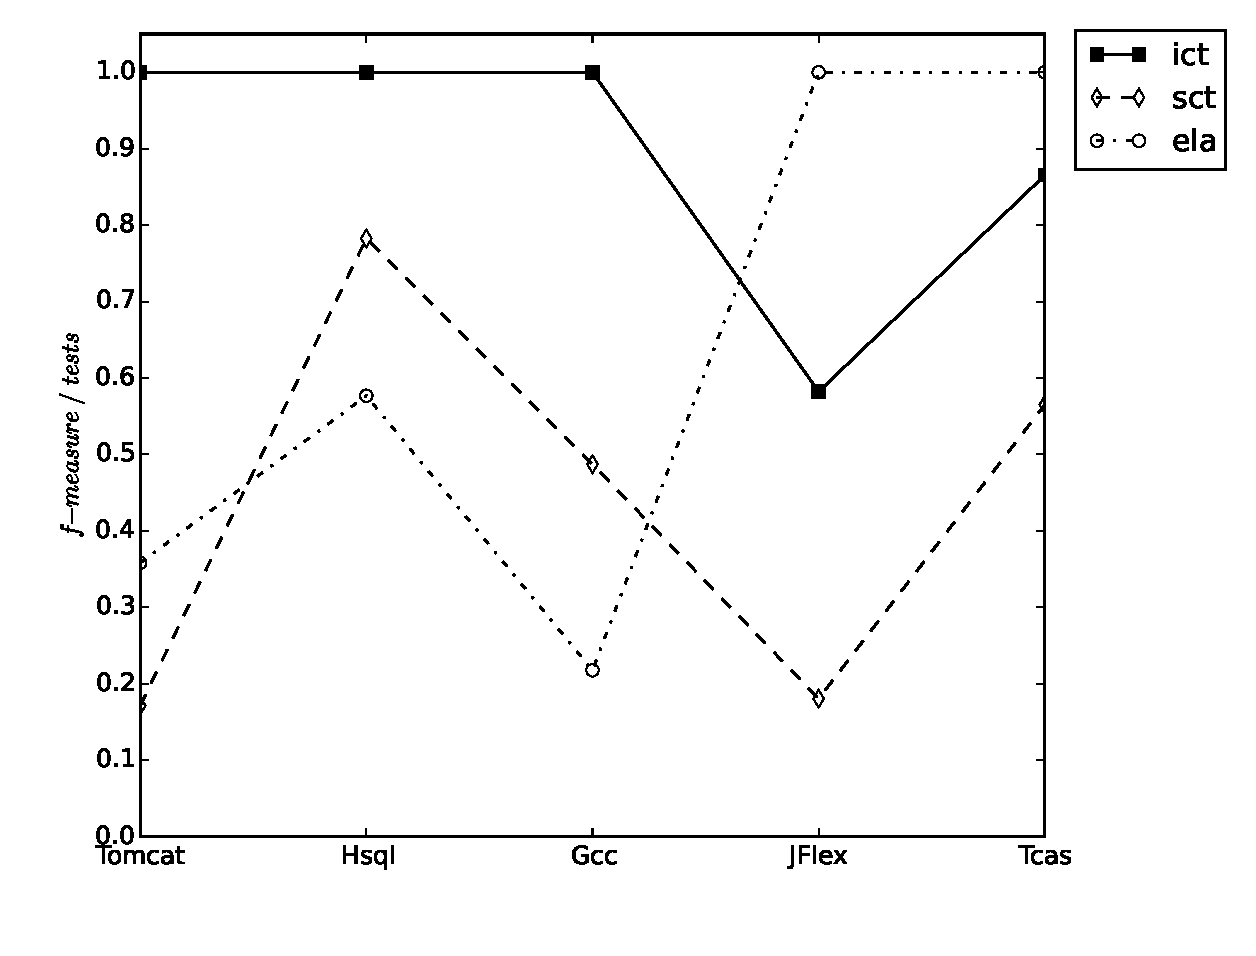
\includegraphics[width=3.4in]{result.eps}
\caption{Comparison of the combining metric}
\label{cm_performance}
\end{figure}

We can learn that \emph{ict} performs better than \emph{sct} for all five subjects.  For \emph{ela}, our approach performs better for three subjects \emph{Tomcat}, \emph{Hsqldb}, and \emph{Gcc}. The reason that our approach does not perform as well as \emph{ela} for subject \emph{JFlex} is that the MFS for that object is a single 2-degree schema (see Table \ref{inputs}), under which ela just needs a 3-way covering array.  For subject \emph{Tcas}, with high-degree MFS as discussed before, our approach is hard to trigger an error with only \emph{2-way}, \emph{3-way}, and \emph{4-way} covering array. As a result, our approach can hardly identify the MFS. Apart from these two special cases, our approach has a significant advantage over the ELA approach.

To summarize, ELA gets the best quality of the MFS, but needs much more test cases than our approach.  It also needs to know the number and degree of the MFS in prior, which limits its application in practice.
%
% there are two shortcomings for the ELA, first, it needed much more test cases that ours, second, it needs to know the number of MFS and the maximal degree of them, which is usually not available in practice.



\subsection{Threats to validity}

There are several threats to validity in our empirical studies. First, our experiments are based on only 5 open-source software. More subject programs are desired to make the results more general. In fact, we plan to conduct comprehensive experiments on the programs with parameters and MFS under control, such that the conclusion of our experiment can reduce the impact caused by specific input space and specific degree or location of the MFS.

Second, there have been many more generation algorithms and MFS identification algorithms. In our empirical studies, we just used AETG \cite{cohen1997aetg} as the test case generation strategy, and OFOT \cite{nie2011minimal} as the MFS identification strategy. As different generation and identification algorithms may affect the performance our proposed CT framework, especially on the number of test cases, some studies for different test case generation and MFS identification approaches are desired.
%For test cases generation, .     But for OFOT, it can significantly accurateness.


%Third, these empirical studies are all on the deterministic condition, i.e., the output of the software are deterministic if their inputs are given. When the output are affected by random events such that we can not determine the output by only one-time execution of the test case, then both the traditional CT process and our new framework do not work. In such a case, to conduct a test case multiple times or introduce some probability in the framework will be of interest.


\section{related works}
Combinatorial testing has been widely applied in practice \cite{kuhn2010practical}, especially on domains like configuration testing \cite{yilmaz2006covering,cohen2006testing,fouche2009incremental} and software inputs testing \cite{cohen1997aetg,borazjany2012combinatorial,garn2014eris}. A recent survey \cite{nie2011survey} comprehensively studied existing works in CT and classified those works into eight categories according to the testing procedure. Based on which, we can learn that test cases generation and MFS identification are two most important parts in CT studies.

%###################qu2008configuration, ghandehari2013applying,

%took a survey on the studies about different aspects of combinatorial testing, and based on which, we can learn that many works in CT focus on separately aspects, i.e. either focus on generation, or on evaluation or on fault localization, or on building models .

Although CT has been proven to be effective at detecting and identifying the interaction failures in SUT, however, to directly apply them in practice can be inefficient and some times even does not work at all. Some problems, e.g., constraints of parameters values in SUT \cite{cohen2007exploiting,cohen2008constructing}, masking effects of multiple failures\cite{dumlu2011feedback,yilmaz2013reducing}, dynamic requirement for the strength of covering array \cite{fouche2009incremental}, will bring many troubles to CT process. To overcome these problems, some works try to make CT more adaptive and flexible.

%Tere are several drawbacks for traditional CT studies. First, not practical, not. To overcome this, several works are proposed to extend CT to make them better application.
%To avoid this,
%the methodology, notions and in CT.
%On this filed, most works separately discussed , such as.

%JieLi \cite{li2012improved} augmented the MFS identifying algorithm by selecting one previous passing test case for comparison, such that it can reduce some extra test cases when compared to another efficient MFS identifying algorithm \cite{zhang2011characterizing}.

S.Fouch{\'e}  et al., \cite{fouche2009incremental} introduced the notion of incremental covering. Different from traditional covering array, it does not need a fixed strength to guide the generation; instead, it can dynamically generate high-way covering array based on existing low-way covering array, which can support a flexible tradeoff between covering array strength and testing resources. Cohen \cite{cohen2007exploiting,cohen2008constructing} studied the impacts of constraints for CT, and proposed an SAT-based approach that can handle those constraints.  Bryce and Colbourn \cite{bryce2006prioritized} proposed an one-test-case-one-time greedy technique to not only generate test cases to cover all the $t$-degree interactions, but also prioritize them according their importance.  E. Dumlu et al., \cite{dumlu2011feedback} developed a feedback driven
combinatorial testing approach that can assist traditional covering in avoiding the masking effects between multiple failures. Yilmaz \cite{yilmaz2013reducing} extended that work by refining the MFS diagnosing method. Specifically, this feedback driven approach firstly generate a $t$-way covering array, and after executing them, the MFS will be identified by utilizing a classification tree method. It then forbidden these MFS and generate additional test cases to cover the interactions that are masked by the MFS. This process continues until all the interactions are covered. Additionally, Nie \cite{nie2013adaptive} constructed an adaptive combinatorial testing framework, which can dynamically adjust the inputs model, strength $t$ of covering array, and generation strategy during CT process.

Our work differs from them mainly in that we proposed a highly interactive framework for test case generation and MFS identification. Specifically, we do not generate a complete $t$-way covering array at first; instead, when a failure is triggered by a test case, we immediately terminate test cases generation and turn to MFS identification. After the MFS is identified, the coverage will be updated and the test cases generation process continues.
%focus on combining two important techniques in CT, i.e., test cases generation and MFS identification, such that the overall cost of CT will be reduced and the identified MFS will be of higher quality.
%


\section{Conclusions}
Combinatorial testing is an effective testing technique at detecting and diagnosis the failure-inducing interactions in the SUT. Traditional CT separately studies test cases generation and MFS identification. In this paper, we proposed a new CT framework, i.e., \emph{interleaving CT}, that integrates these two important stages, which allows for both generation and identification better share each other's information. As a result, interleaving CT approach can provide a more efficient testing than traditional sequential CT.

Empirical studies were conducted on five open-source software subjects. The results show that with our new CT framework, there is a significant reduction on the number of generated test cases when compared to the traditional sequential CT approach, while there is no decline in the quality of the identified MFS. Further, when comparing with the ELA \cite{martinez2009locating,martinez2008algorithms}, our approach also performed better, especially with fewer test cases.

As a future work, we need to extend our interleaving CT approach with more test case generation and MFS identification algorithms, to see the extent on which our new CT framework can enhance those different CT-based algorithms. Another interesting work is to combine interleaving CT approach with white-box testing techniques, so that it can provide more useful information for developers to debug the system.


%\end{document}  % This is where a 'short' article might terminate

%ACKNOWLEDGMENTS are optional
%\section{Acknowledgments}
%This section is optional; it is a location for you
%to acknowledge grants, funding, editing assistance and
%what have you.  In the present case, for example, the
%authors would like to thank Gerald Murray of ACM for
%his help in codifying this \textit{Author's Guide}
%and the \textbf{.cls} and \textbf{.tex} files that it describes.

%
% The following two commands are all you need in the
% initial runs of your .tex file to
% produce the bibliography for the citations in your paper.
\bibliographystyle{abbrv}
%\bibliographystyle{unsrt}
\bibliography{sigproc}  % sigproc.bib is the name of the Bibliography in this case
% You must have a proper ".bib" file
%  and remember to run:
% latex bibtex latex latex
% to resolve all references
%
% ACM needs 'a single self-contained file'!
%
%APPENDICES are optional
%\balancecolumns
%\appendix
%%Appendix A
\end{document}
